\documentclass[modern]{aastex62}
\usepackage{amsmath}
\graphicspath{{./}{figures/}}

% typography
\setlength{\parindent}{1.\baselineskip}
\newcommand{\acronym}[1]{{\small{#1}}}
\newcommand{\project}[1]{\textsl{#1}}
\newcommand{\package}[1]{\textsl{#1}}
\newcommand{\gaia}{\textsl{Gaia}}
\newcommand{\pans}{\textsl{Pan-STARRS}}
\newcommand{\DR}[1]{\acronym{DR#1}}
\newcommand{\todo}[1]{{\color{red} TODO: #1}}

% astronomy stuffs
\newcommand{\msun}{\textrm{M}_\odot}
\newcommand{\kpc}{\textrm{kpc}}
\newcommand{\kms}{\ensuremath{\textrm{km}~\textrm{s}^{-1}}}
\newcommand{\bs}[1]{\boldsymbol{#1}}
\newcommand{\masyr}{\ensuremath{\textrm{mas}~\textrm{yr}^{-1}}}
\newcommand{\feh}{\ensuremath{[\textrm{Fe} / \textrm{H}]}}
%\newcommand{\kms}{\mbox{km s$^{-1}~$}} 
\newcommand{\kmse}{\mbox{km s$^{-1}$}} 
\newcommand{\vlsr}{$V_{\rm LSR}~$}
\newcommand{\vlsre}{$V_{\rm LSR}$}
\newcommand{\hi}{H{\footnotesize I} }
\newcommand{\hie}{H{\footnotesize I}}
\newcommand{\lms}{$L_{\rm MS}~$}
\newcommand{\lmse}{$L_{\rm MS}$}
\newcommand{\bms}{$B_{\rm MS}~$}
\newcommand{\bmse}{$B_{\rm MS}$}

\newcommand{\clustername}{\textsl{NAME}}

%% Reintroduced the \received and \accepted commands from AASTeX v5.2
% \received{January 1, 2018}
% \revised{January 7, 2018}
% \accepted{\today}

\submitjournal{ApJ}
\shorttitle{Sample article}
\shortauthors{People et al.}

\begin{document}

\title{A young cluster in the Galactic halo: \\
Recent star formation associated with the Magellanic stream}

\author{Author McAuthorface}
\affil{Some affiliation}

\author[0000-0003-0872-7098]{Adrian~M.~Price-Whelan}
\affiliation{Department of Astrophysical Sciences,
             Princeton University, Princeton, NJ 08544, USA}
\email{adrn@astro.princeton.edu}
\correspondingauthor{Adrian M. Price-Whelan}

\author[0000-0002-1793-3689]{David L. Nidever}
\affiliation{Department of Physics, Montana State University, P.O. Box 173840, Bozeman, MT 59717-3840, USA}
\affiliation{National Optical Astronomy Observatory, 950 North Cherry Ave, Tucson, AZ 85719}


\author[0000-0003-1680-1884]{Yumi Choi}
\affiliation{Department of Physics, Montana State University, P.O. Box 173840, Bozeman, MT 59717-3840, USA}
\affiliation{Steward Observatory, University of Arizona, 933 North Cherry Avenue, Tucson AZ, 85721}


\begin{abstract}

We report the discovery of a young ($\lesssim 100~\textrm{Myr}$), metal-poor ($[\textrm{Fe}/\textrm{H}] \sim -1$) star cluster in the halo of the Milky Way. 
The cluster --- \clustername\ --- is likely associated with the leading arm of the gas stream emanating from the Magellanic cloud system and is located $\approx 60^\circ$ from the LMC center, on the other side of the Milky Way disk relative to the LMC.
By assuming the cluster is co-located with HI gas in the stream, we, for the first time, directly measure the distance to the Magellanic stream, $d \approx 25~\textrm{kpc}$. 
At this location relative to the LMC, this distance is inconsistent with predictions from models of the LMC/SMC interaction and infall into the Milky Way.
The estimated age of \clustername\ is consistent with the time of last passage through the Galactic midplane. 
We therefore conclude that this star-formation event was triggered by the last disk passage, which occurred at a Galactocentric radius $R \approx XX~\kpc$.

\end{abstract}

\keywords{Galaxy: halo}


\section{Introduction} \label{sec:intro}

The stellar halo of the Milky Way is characterized by its old ($\approx XX$--$YY~\textrm{Gyr}$), metal-poor ($\feh \approx -1.5$) stellar population.
This is understood as a signature of the dominant (in stellar mass) progenitor systems that were accreted and disrupted early on in the Milky Way's formation: massive dwarf galaxies (cite deason, etc.).
The 
(Built up from destroyed satellites that lost their gas on infall)

However, the Milky Way continues to accrete satellite galaxies, as is evidenced by the prominent stellar stream from the Sagittarius dwarf galaxy that can be traced $>360^\circ$ in angle, and the presence of the Magellanic cloud system.
While Sagittarius was likely stripped of its neutral gas long ago (cite), the LMC/SMC system contains $\approx XX~\msun$ of HI gas (cite), which form leading and trailing gas streams that cover $\approx 200^\circ$ on the sky.
(Gas is great, can run models to try to reproduce. But lacks distance information)
(Many people search for stars associated with the stream, but must be diffuse)


\section{Data and cluster discovery} \label{sec:data}

We use astrometric data from the \gaia\ mission (\citealt{Prusti:2016}), data release 2 (\DR{2}; \citealt{Gaia-Collaboration:2018, Lindegren:2018}) cross-matched to the \pans\ data release 1 photometry ($griz$ magnitudes; \citealt{Chambers:2016}) to search for distant, comoving multiplets of blue stars.\footnote{We use the cross-match provided by the \gaia\ science archive at \url{https://gea.esac.esa.int/archive/}.}
In detail, we initially query all stars from the \gaia--\pans\ cross-match that have $(g - i) < 1$, parallax $\varpi < 1~{\rm mas}$, and Galactic latitude $|b| > 10^\circ$.

Figure \ref{fig_skypm} shows the spatial and proper motion distribution in the region of interest with the objects in
a small proper motion selection shown as black and red dots.  The color magnitude diagram (CMD) of the same objects
is shown in Figure \ref{fig_cmd} and clearly reveals a sequence of objects that follow the shape of a young main-sequence.
The PS1 photometry of the same region is shown in Figure \ref{fig_isochrone} and as well as young, metal-poor isochrones at
a distance of 25 kpc.  Finally, Figure \ref{fig_gass} shows a position-velocity diagram at the position of the cluster of the \citep[GASS;][]{McClure-Griffiths2009} \hi data that has been Gaussian decomposed using the technique in \citet{Nidever2008}.
The component of the LA II can be seen on the left-hand side of the figure and a similar \hie stream can be seen near the
position of the cluster.


\section{Results} \label{sec:results}

We have used the new Gaia data to detect a young, metal-poor cluster in the halo of the Milky Way at a distance of 25 kpc and
a Milky Way z-height of 12 kpc.  The detection of such a young cluster so far from the star-forming disks of any nearby
galaxy is highly unusual.  However, the proximity of the new cluster to the Leading Arm of the Magellanic Stream suggests
that the cluster originated from this metal-poor gas \citep{Fox2018}.  Previously studies have detected young stars in the Leading Arm and gas in the periphery of the Magellanic Clouds \citep{Casetti-Dinescu2014,MoniBidin2017}, however, this is the first time
that an entire star cluster has been detected so far from the Clouds.  

We evaluate the hypothesis that the cluster formed in the Leading Arm.  The mean proper motion values in the Magellanic Stream
coordinate system \citep{Nidever2008} are ($\mu_{\rm MSL}$,$\mu_{\rm MSB}$)=($+$1.X,0.X) mas yr$^{-1}$ which is very similar to the
mean values of the LMC and SMC with ($+$1.X,0.X) mas yr$^{-1}$ and ($+$1.X,0.X) mas yr$^{-1}$, respectively.  The simulations
of \citet{Besla2012} also predict proper motions at this position of approximately ($+$1.X,0.X) mas yr$^{-1}$.  The Magellanic Stream
simulations give distances of the Leading Arm at this position of $\sim$50 kpc, however, many of these do not include the
effects of ram pressure from the hot MW halo which could cause the gas to drop in its orbit to smaller Galactocentric
distances (NEED TO DOUBLE-CHECK THIS).  In addition Figure \ref{fig_gass} shows that there is Leading Arm \hi~gas at the
position of the position of the cluster with a velocity of \vlsr=70 \kmse.



\begin{figure}
\centering
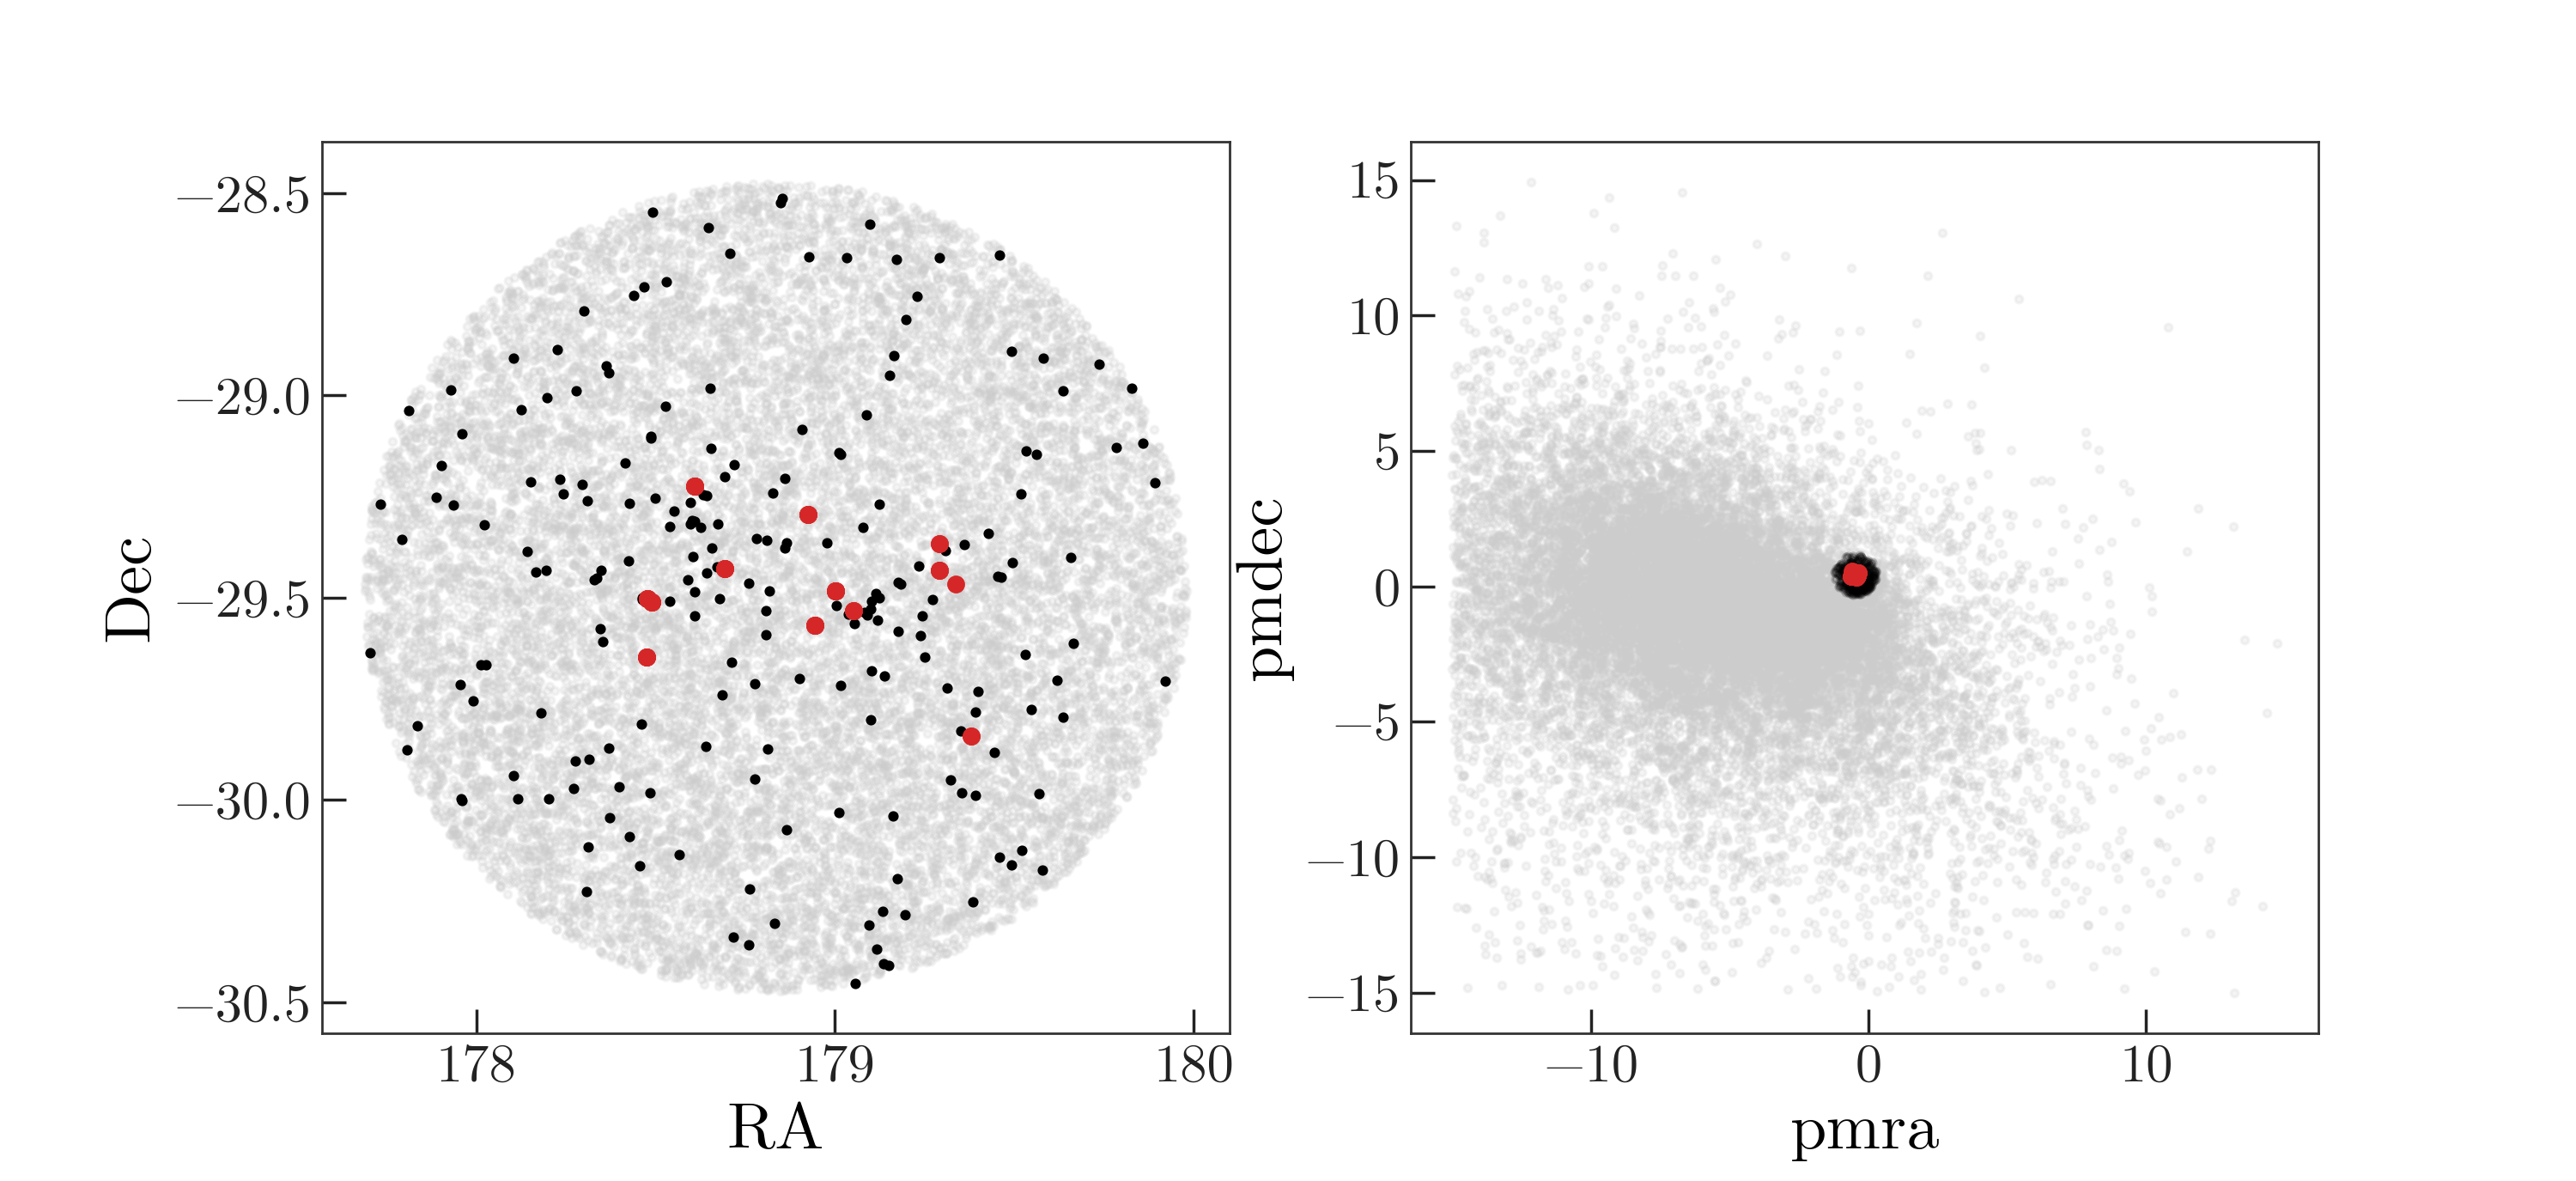
\includegraphics[width=12cm]{sky_pm.png}
\caption{Figure 1}  
\label{fig_skypm}
\end{figure}

\begin{figure}
\centering
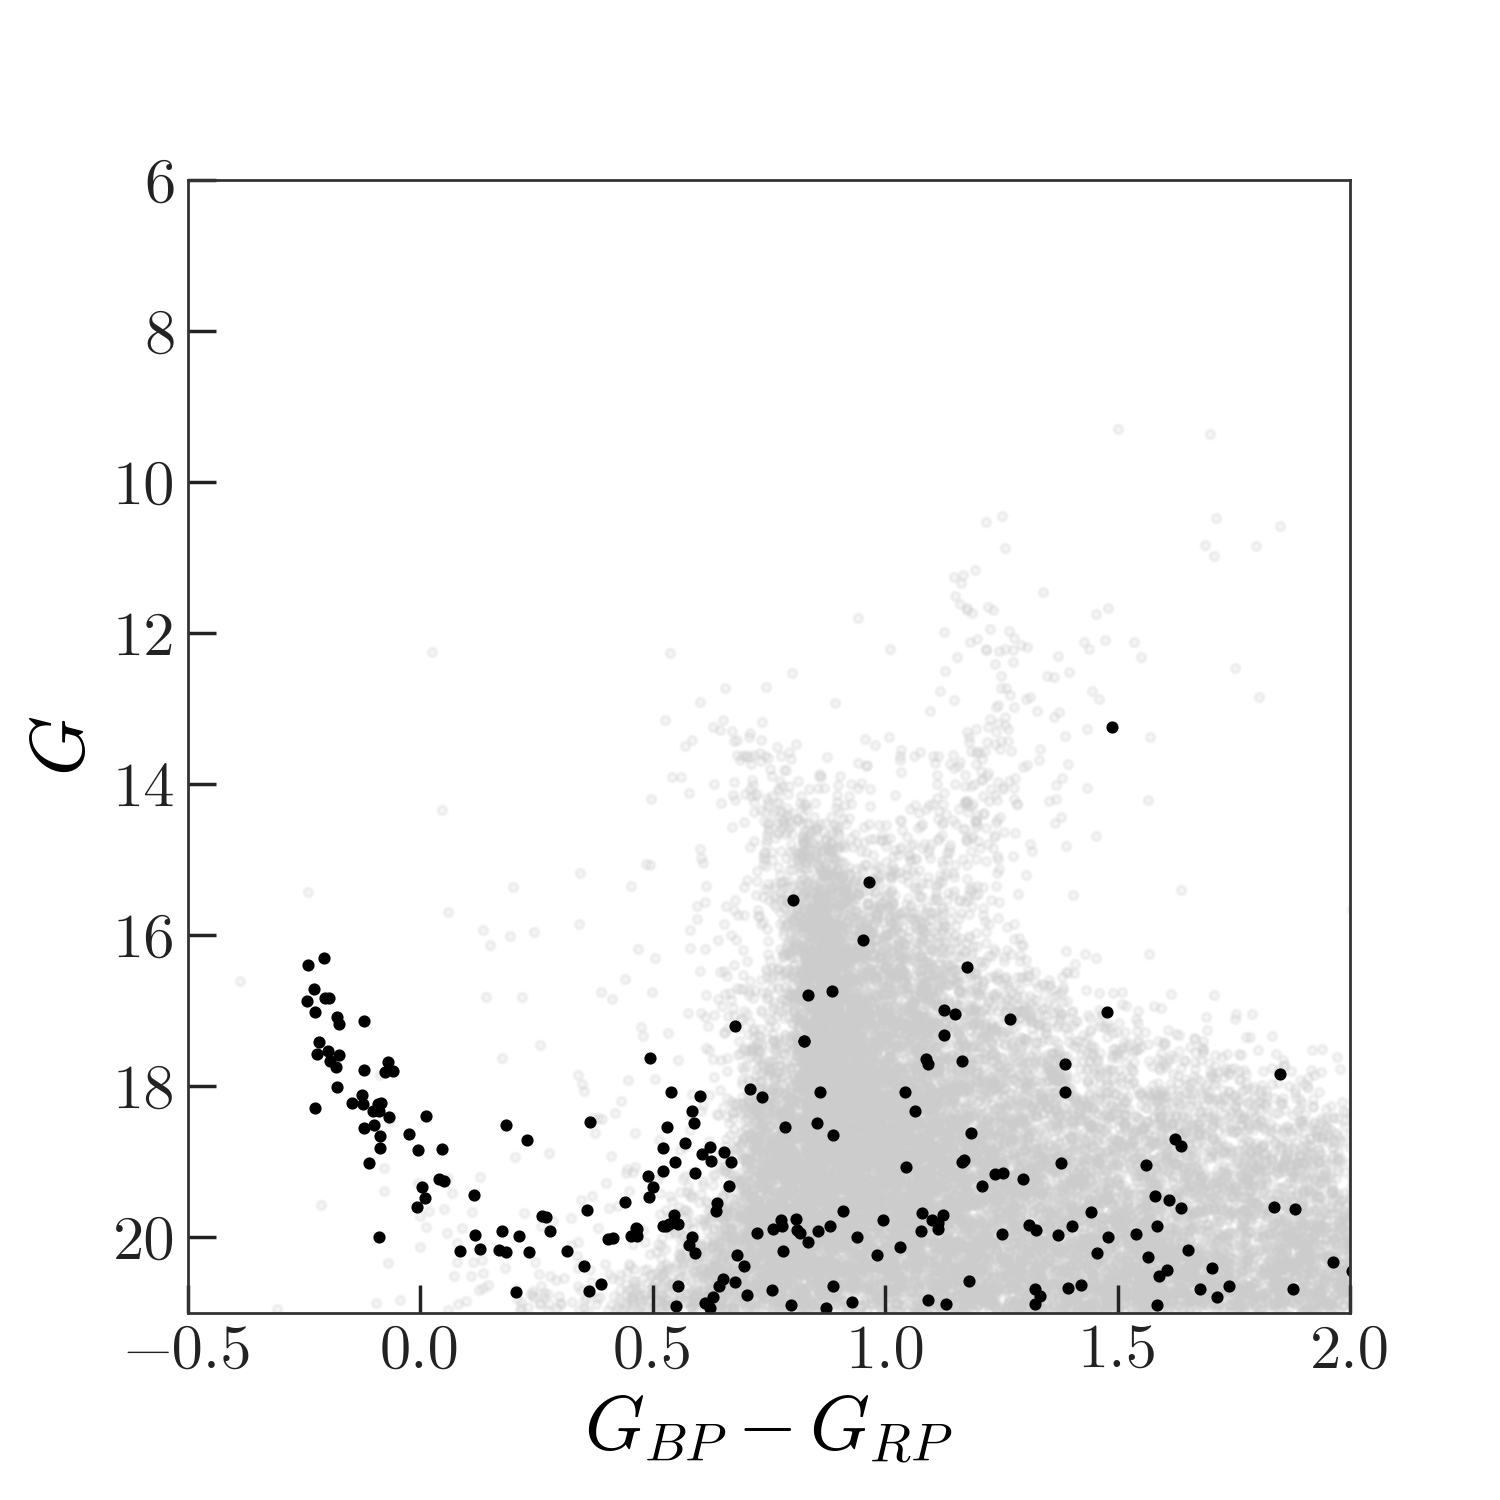
\includegraphics[width=8cm]{cmd.png}
\caption{The Gaia DR2 color magnitude diagram of the region showing the pronounced
young stellar main sequence.}
\label{fig_cmd}
\end{figure}

\begin{figure}
\centering
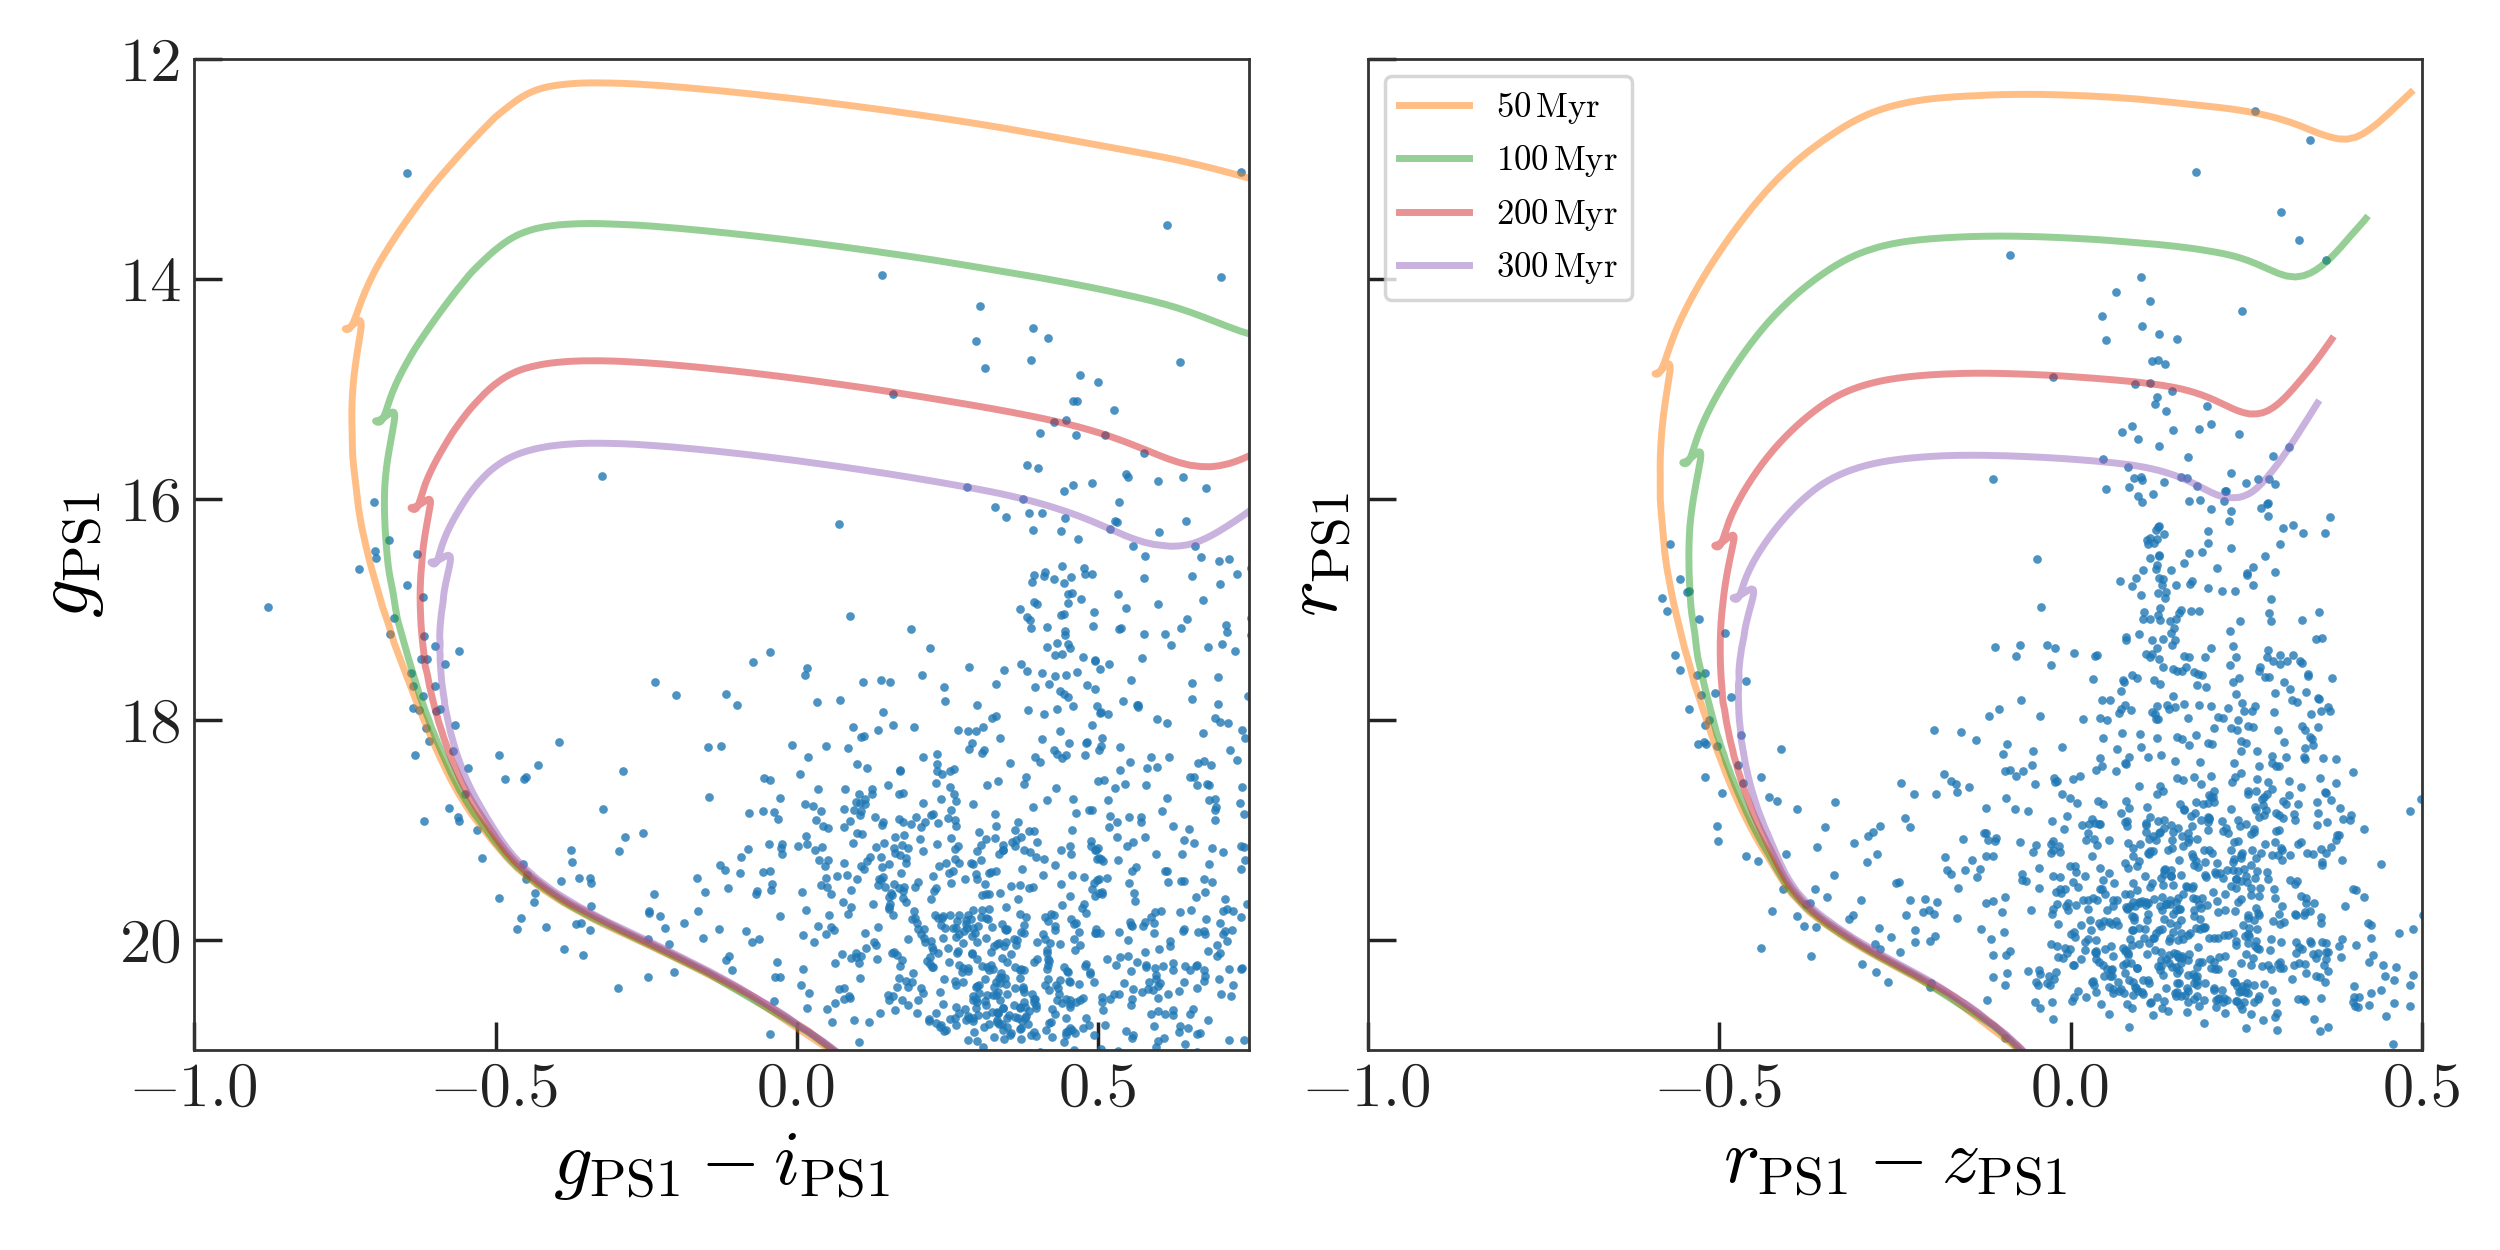
\includegraphics[width=8cm]{isochrone.png}
\caption{PS1 color magnitude diagrams with young, metal-poor (\feh=-1.0) isochrones overplotted at
a distance of 25 kpc.}
\label{fig_isochrone}
\end{figure}

\begin{figure}
\centering
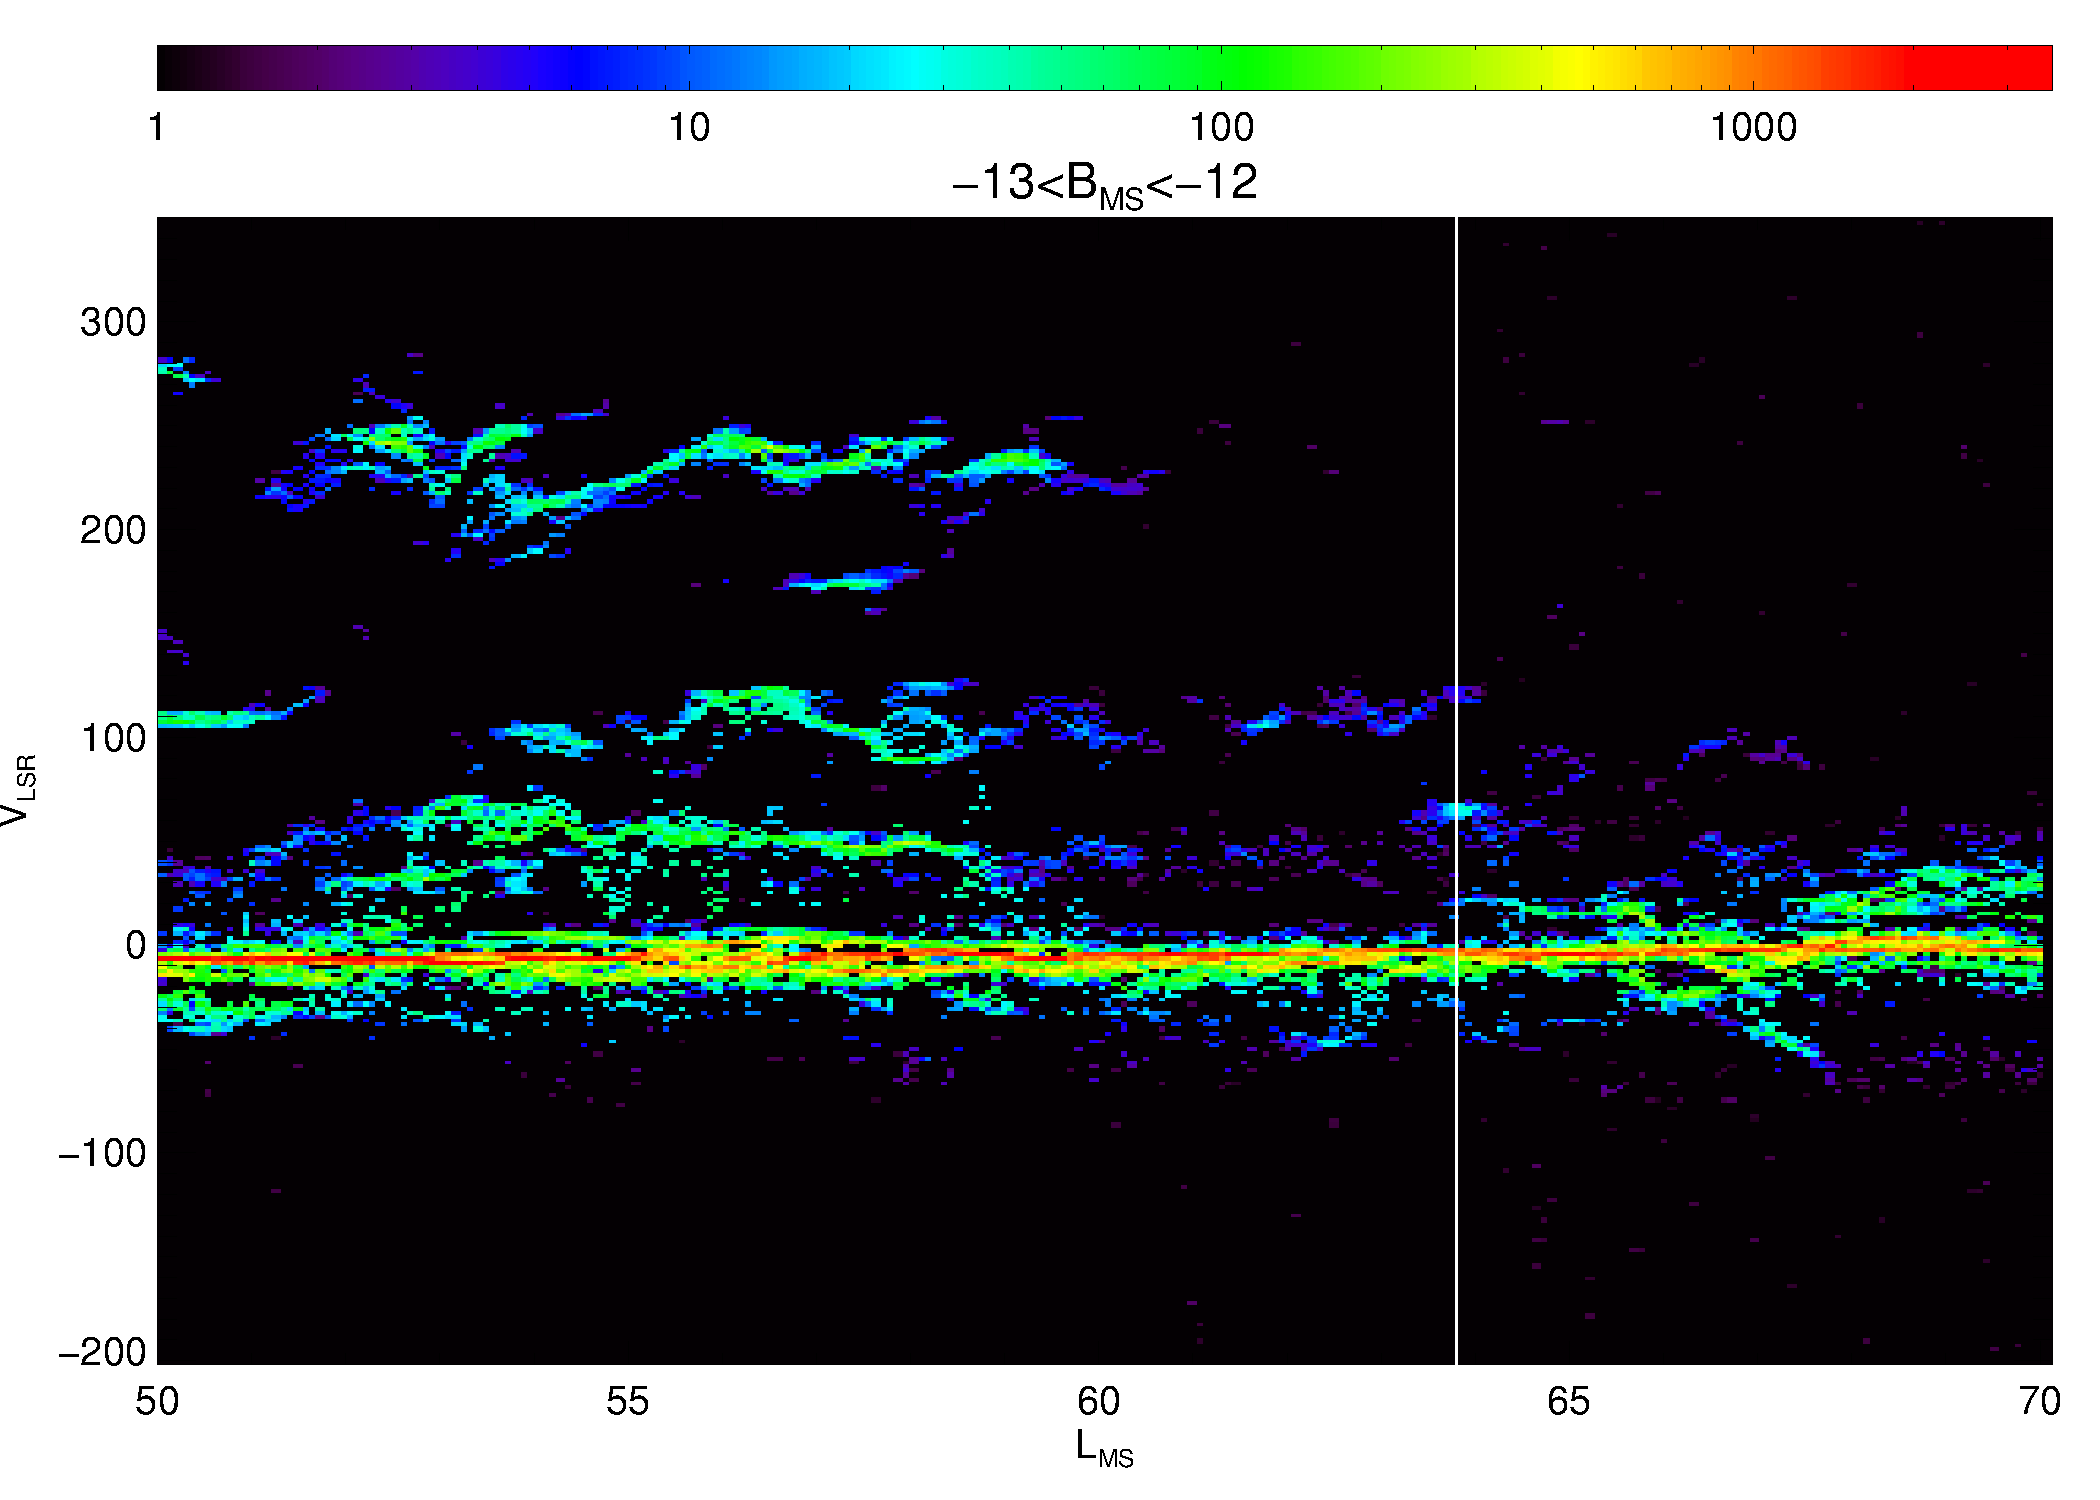
\includegraphics[width=8cm]{gass_vlsrmlon.pdf}
\caption{GASS position-velocity diagram.}
\label{fig_gass}
\end{figure}

\begin{figure}
\centering
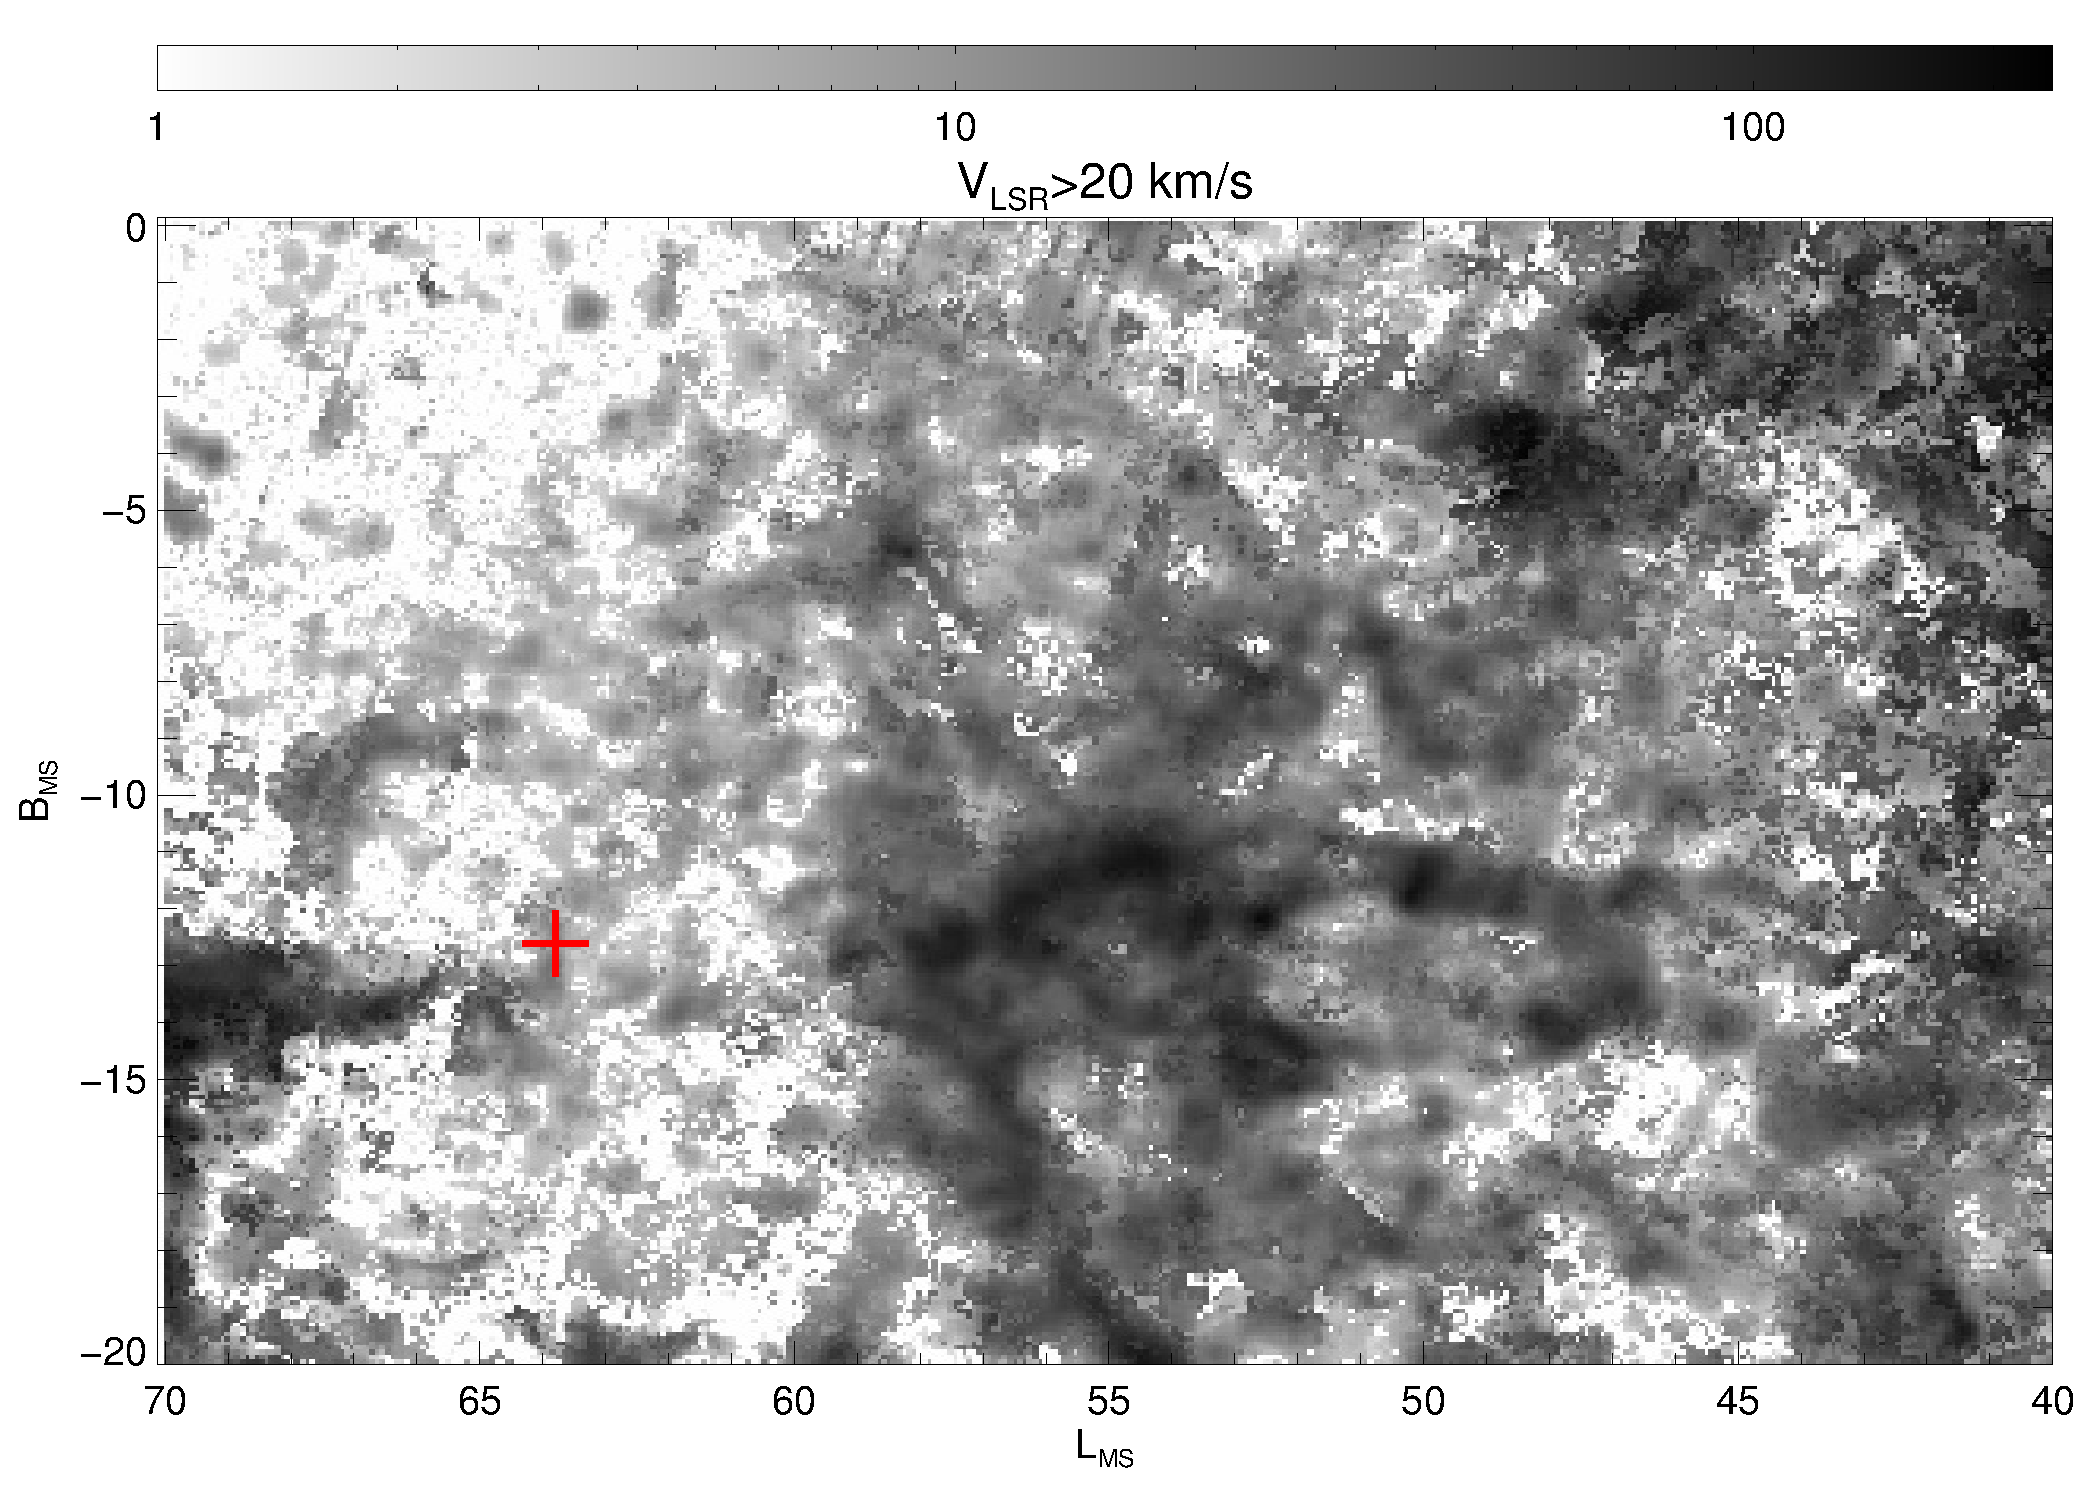
\includegraphics[width=8cm]{gass_mlatmlon.pdf}
\caption{GASS \hi column density in the region of LA II. The red cross marks the position
of the young cluster.}
\label{fig_gass}
\end{figure}

\begin{figure}
\centering
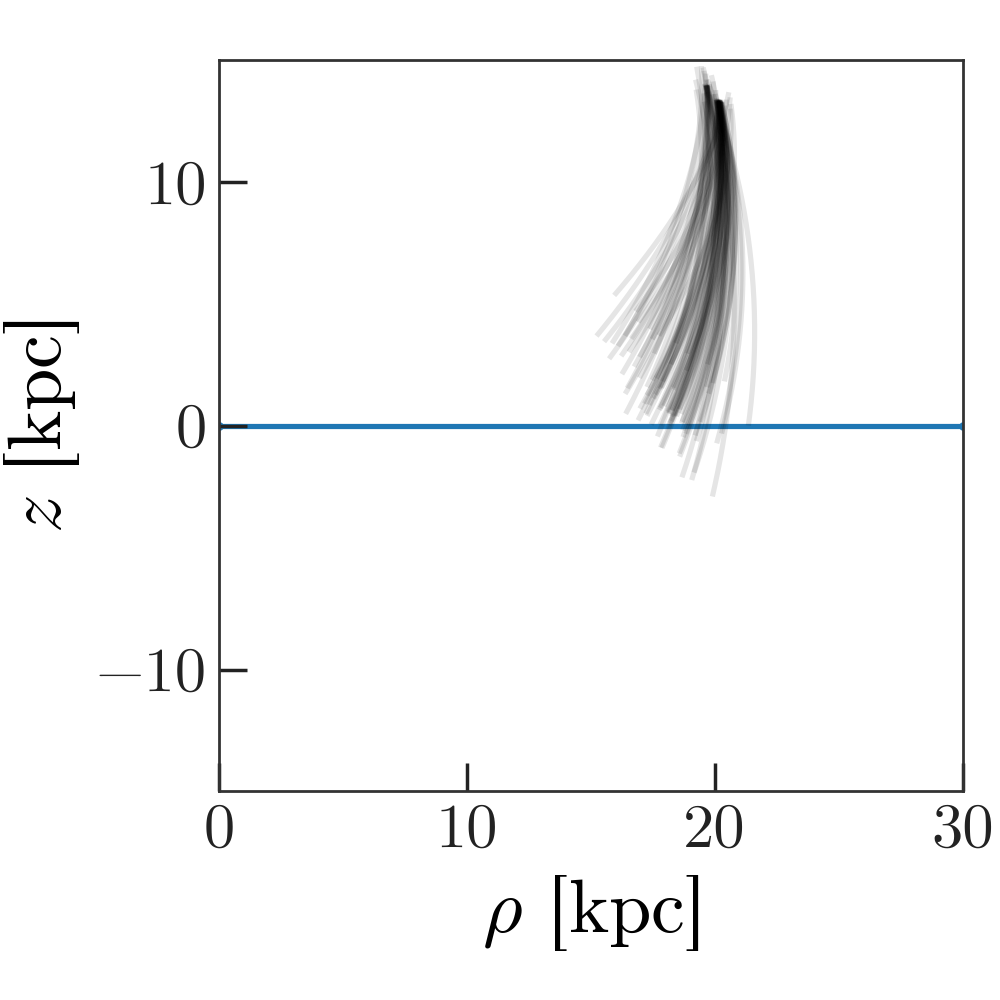
\includegraphics[width=8cm]{orbits.png}
\caption{Integrated orbits (over 60 Myr) of the star cluster using the Gaia DR2 proper motions, the
\hi~velocity and a distance of 25 kpc.  The orbits intersect the MW midplane about 
60 Myr ago which is close to the age of the cluster.}
\label{fig_gass}
\end{figure}

\section{Discussion} \label{sec:discussion}

- Streams or clusters in the halo from star-formation from Sgr or dwarf gas

- Sgr young globular clusters: same thing as this? Indication of when Sgr lost its gas?

\section{Conclusion} \label{sec:conclusion}


\acknowledgments

We thank some people...

This work has made use of data from the European Space Agency (ESA)
mission {\it Gaia} (\url{https://www.cosmos.esa.int/gaia}), processed by
the {\it Gaia} Data Processing and Analysis Consortium (DPAC,
\url{https://www.cosmos.esa.int/web/gaia/dpac/consortium}). Funding
for the DPAC has been provided by national institutions, in particular
the institutions participating in the {\it Gaia} Multilateral Agreement.

\vspace{5mm}
\facilities{TODO}

\software{
    \package{Astropy} \citep{astropy},
    \package{dustmaps}\footnote{\url{https://github.com/gregreen/dustmaps}},
    \package{gala} \citep{gala},
    \package{IPython} \citep{ipython},
    \package{matplotlib} \citep{mpl},
    \package{numpy} \citep{numpy},
    \package{scipy} \citep{scipy}
}

\bibliographystyle{aasjournal}
\bibliography{ms}

\end{document}
